\chapter{问题定义}\label{chapter:def}
在第\ref{chapter:architecture}章介绍系统架构之前,本章先定义需要解决的问题。

\section{数据结构}
要存储的目标数据被称为blob,它是一个没有子结构和含义的二进制数据块。上层应用在
写入数据之前,需要先将待存储的数据转换成二进制数据块,再调用接口函数将数据写入
服务器。读出数据之后,系统直接将二进制数据块返回给上层应用,具体的解析工作由上
层应用完成。这样设计的优点,一是可以简化系统实现,从而提高执行效率;二是使系统
的应用范围更广泛,由于任何数据在计算机内的终极存储表示都是二进制数据块,所以理
论上该系统可以支持任何应用。这样设计的缺点是降低了系统的易用性,需要上层应用完
成更多的序列化/解析工作。\footnote{在当前实验条件下,高效和普适性比易用性更重
要。}

每一个blob拥有一个字符串类型的ID,称作blobID。多个blob逻辑上被划在一个``桶''
中,这通过给每个blob附加另一个字符串类型的ID实现,该ID被称作bucketID,如图
\ref{figure:datastructure}所示。所有具有相同bucketID的blob被认为装在同一个桶
中,同一个桶中的blobID是唯一的,不同桶中的的不同blob则可能具有相同的blobID。这
样,对于blob的索引是通过给出两级ID实现的。与最基本的分布式哈希表相比,多出的一
级ID实际上维护了数据之间的\emph{归类}关系,即按照bucketID是否相同将数据归入不
同的类别。
\begin{figure}[htb]
  \centering
  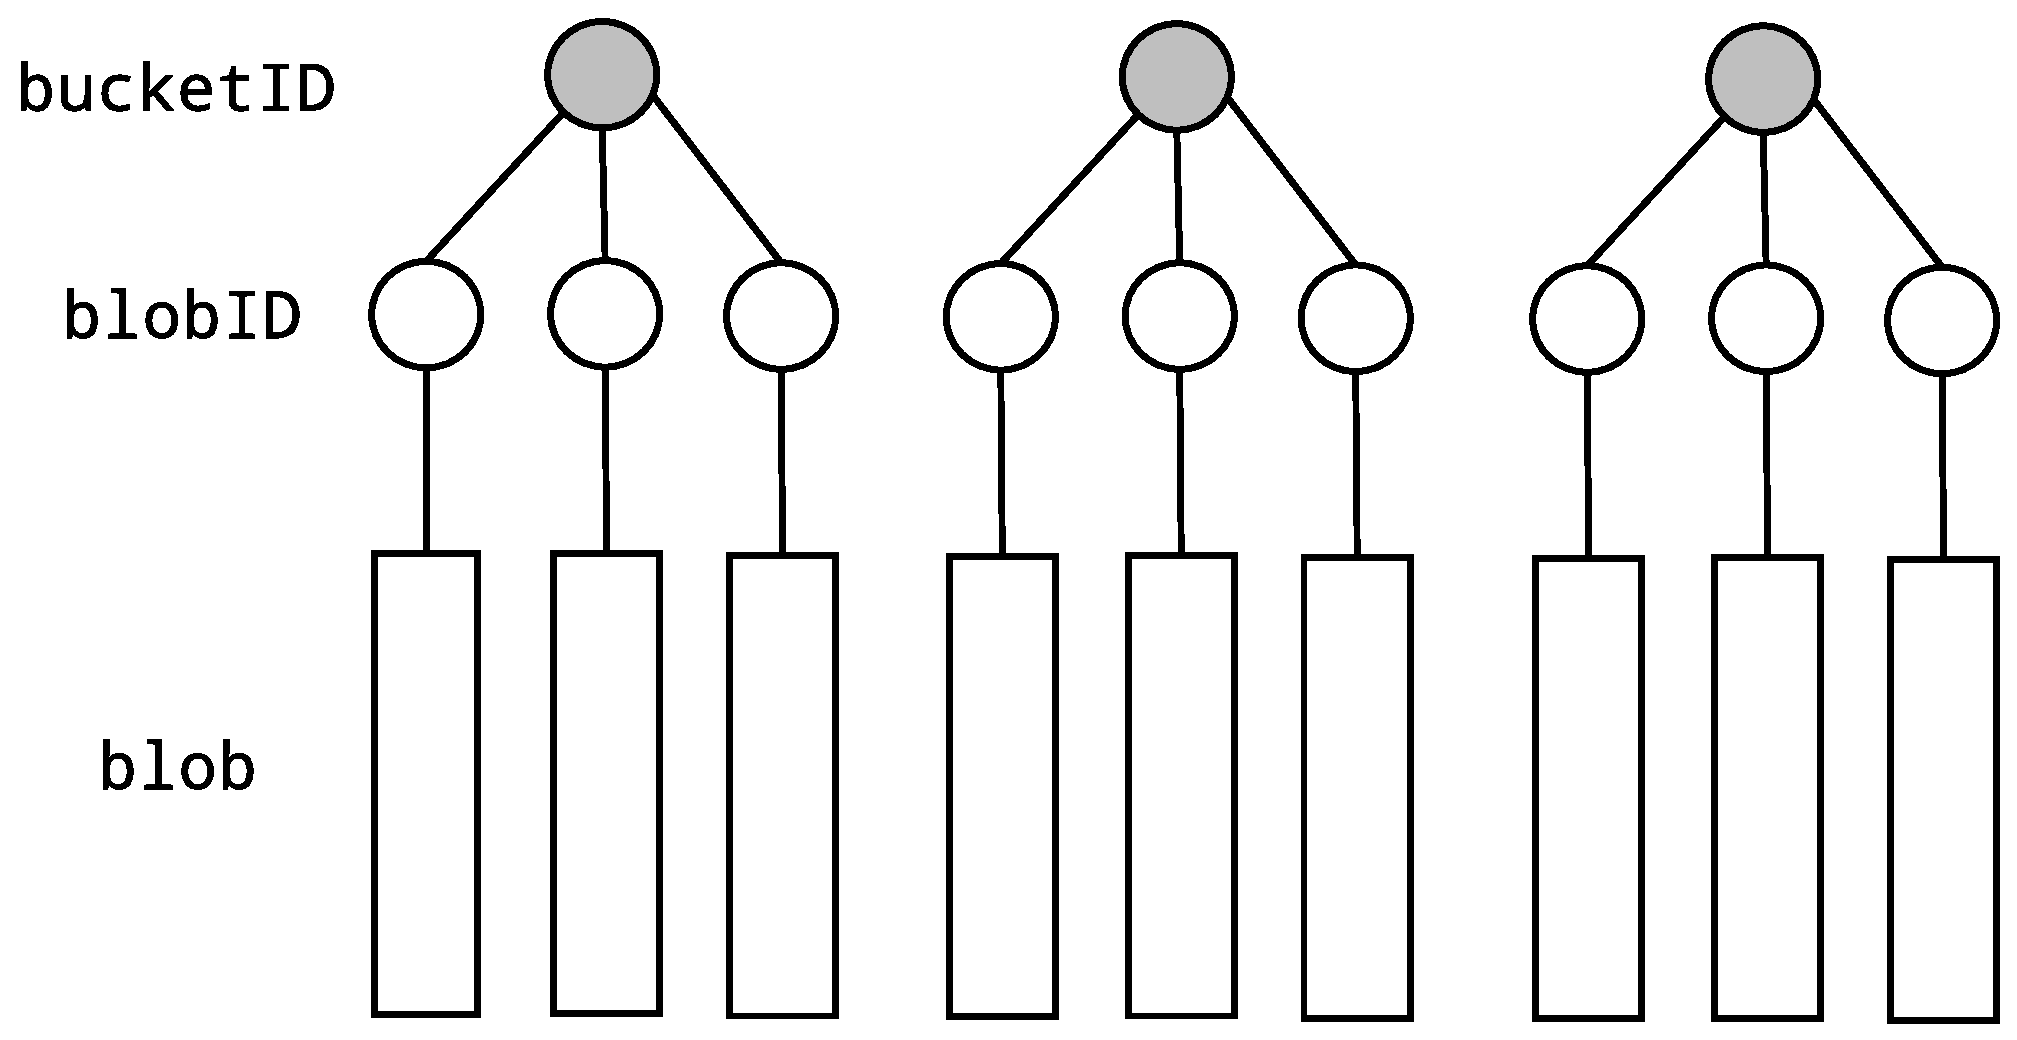
\includegraphics[width=1.0\linewidth]{datastructure}
  \caption[分布式二级哈希表数据结构]{分布式二级哈希表数据结构。每个blob拥有一
  个blobID和一个bucketID。共享相同bucketID的多个blob被归为同一类。}
  \label{figure:datastructure}
\end{figure}

\section{接口}\label{section:api}
分布式二级哈希表作为各种云存储应用的底层存储后端,为不同的应用提供了统一的调用
接口。接口的设计既要保证通用性,考虑系统实现的效率,又不能损失易用性。分布式哈
希表的调用接口及说明参见表\ref{table:api}。

\begin{table}[htb]
  \centering
  \caption[分布式二级哈希表调用接口及说明]{分布式二级哈希表调用接口及说明。这
  些接口是分布式二级哈希表为上层应用提供的调用接口,以标准C语法为例。}
  \label{table:api}
  \begin{tabular}{p{5cm}|p{9cm}}
    \toprule[1.5pt]
    \hei 函数原型 & \hei 说明 \\
    \midrule[1pt]
    int createBucket(const char *bucketID); &
    创建一个空桶,该桶内不包含任何blob。当用户刚刚注册云存储服务时,可以调用此
    函数。\\
    \midrule[1pt]
    int deleteBucket(const char *bucketID); &
    删除一个桶中的所有blob。当用户注销删除账户全部数据时,可以调用此函数。\\
    \midrule[1pt]
    int existBucket(const char *bucketID); &
    查看一个桶是否存在。当需要查看一个用户是否存在时,可以调用此函数。\\
    \midrule[1pt]
    int deleteBlob(const char *bucketID, const char *blobID); &
    删除一个blob。当需要删除用户的某个特定数据时,可以调用此函数。\\
    \midrule[1pt]
    int existBlob(const char *bucketID, const char *blobID); &
    查看一个blob是否存在。当需要查看用户的某个特定数据是否存在时,可以调用此函
    数。\\
    \midrule[1pt]
    int loadBlob(const char *bucketID, const char *blobID, int *blobLength,
    void *blob); &
    读取某个blob的内容。当需要读取用户的某个特定数据时,可以调用此函数。\\
    \midrule[1pt]
    int saveBlob(const char *bucketID, const char *blobID, const int
    blobLength, const void *blob); &
    将blob存入服务器,覆盖具有相同索引的数据。当需要存储或更新用户的某个特定数
    据时,可以调用此函数。\\
    \bottomrule[1.5pt]
  \end{tabular}
\end{table}

由于分布式二级哈希表可能为多个上层应用提供存储服务,因而每一个独立的应用在使用
分布式二级哈希表之前需要先创建一个服务实例\footnote{类似MFC中的HANDLE}。在调用
具体的接口函数时,此实例也要作为一个参数传递给系统。出于简化的目的,本论文的叙
述将略去关于实例的说明,只考虑仅有一个实例的情况。

\section{实验假设}\label{section:assumption}
任何一个系统都不可能解决所有的问题,分布式二级哈希表也不例外。下面的假设在很大
程度上影响了系统架构的设计:
\begin{enumerate}
  \item 单个blob的大小在1KB到1MB左右。具备这个规模数据的最典型应用是文本系统。
  比如个人邮件的文本部分,不包括附件和多媒体等内容,尺寸一般小于一兆字节。问答
  系统和论坛留言也大致如此。此外,矢量图和尺寸较小的压缩图也属于这个尺寸范围。
  这些应用一般只要求知道数据属于哪个用户,至于数据之间的关系则没有过多要求,而
  且一般由上层应用自己来维护关系信息,因此分布式二级哈希表可以很好的满足这些应
  用的存储需求。另一方面,虽然单个数据的尺寸不大,但是数据的总量可能很大。这就
  要求系统的算法复杂度不能太高,能在海量数据中迅速定位到指定的目标。后面我们会
  看到,由于采用了哈希算法,数据的定位复杂度是O(1),能够保证系统在应对海量数据
  请求时保持较高的执行效率。
  \item 存储服务器集群的规模大概是50台上下,每一台服务器的硬盘容量在1TB左右。
  由于该系统的集群规模与典型数据中心相差甚远,机器的故障发生率并不频繁,
  \cite{hastorun2007dynamo}可以假设大部分时间所有机器都是正常运转的。另一方
  面,机器故障也是有可能发生的。如果数据大部分时间保存在内存中,则需要系统定期
  将数据写入硬盘以应对系统错误;如果数据大部分时间保存在硬盘上,则需要利用数据
  局部性在内存中构建数据缓存以提高效率。为了解决硬盘发生错误带来的灾难性后果,
  我们还需要将数据进行备份,即在多台服务器上存储同一数据的多个副本。也就是说,
  同样的操作需要在多台存储服务器上进行。比如,上层应用调用了分布式哈希表的写入
  函数,假设数据在系统中有了三个副本,那么系统需要向这三台服务器发送写请求。这
  里系统需要解决的一个关键问题是如何保证副本间的数据一致性。强一致性要求数据在
  不同副本之间总是相同的,但是理论界和工业界普遍认可实现强一致性不仅技术难度较
  大,这样的系统运行效率也往往很低。\cite{fox1997cluster}与之相对的另一种解决
  方案是弱一致性,它不保证数据的不同副本总是完全相同的,而是保证读出的数据总是
  最近一次写入的数据。本质上讲,系统可以利用数据从开始写入到最终读出之间的时间
  间隔实现数据在不同副本之间的同步,因而操作的平均响应时间大大缩短,而吞吐率则
  得以提高。
  \item 要求系统在饱和运转时,操作成功率大于99.999\%,每台服务器平均每秒处理请
  求不小于50左右,平均响应时间在百毫秒数量级。当系统要应对大量数据请求时,由于
  处在高负荷运转状态,系统的响应时间会降低。要在保证系统正确性的前提下,尽量提
  高系统的运行效率。
  \item 系统由标准C代码实现。存储服务器上运行Linux操作系统,使用标准C代码实现
  分布式二级哈希表既保证了系统的运行效率,又不会影响代码的可移植性。
  
\end{enumerate}
